\subsection{Layer Hardware}
The music amplification layer hardware consists of the Arduino Uno and the 6 haptic motor controllers.

\subsection{Layer Operating System}
As previously mentioned, the code for mapping the soundwaves/vibrations to the haptic motors will be embedded into the firmware of the Arduino Uno, so no other operating system should be necessary.

\subsection{Layer Software Dependencies}
There are drivers available for download with the haptic motors (from the website they were purchased from), which are needed to properly control output to the motors.

\subsection{Subsystem 1}
This subsystem consists of the motors connecting with the Arduino Uno.

\begin{figure}[h!]
	\centering
 	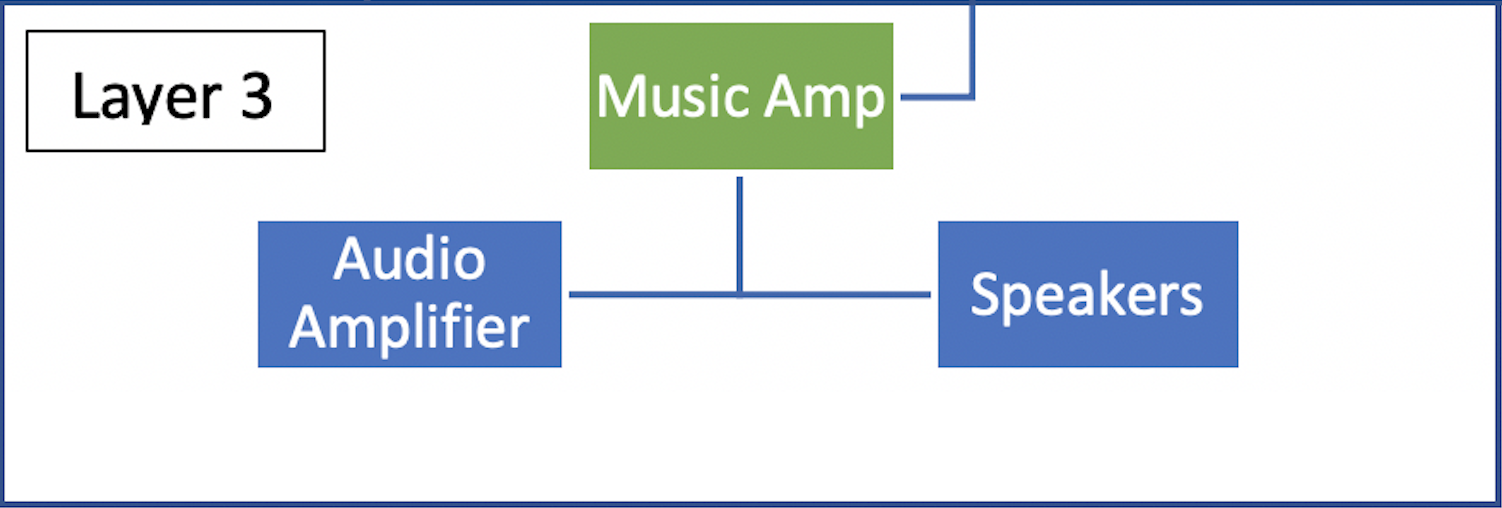
\includegraphics[width=0.60\textwidth]{architectural design specification latex/images/subsystem3.png}
 \caption{Example subsystem description diagram}
\end{figure}

\subsubsection{Subsystem Hardware}
The hardware for this subsystem is the 6 haptic motor controllers, the Arduino Uno, and any required wiring. The motors will be embedded within the vest.

\subsubsection{Subsystem Operating System}
No operating system is needed.

\subsubsection{Subsystem Software Dependencies}
There are drivers that may need to be installed onto the Arduino Uno in order to properly control the haptic motors.

\subsubsection{Subsystem Programming Languages}
The Arduino Uno code provided by the motor sellers is in Python.

\subsubsection{Subsystem Data Structures}
After being filtered, the signals are received by the Arduino and are then converted to voltages, depending on the type of signal (lows/mids/highs), and within a range of 2V - 5V.

\subsubsection{Subsystem Data Processing}
The voltages are mapped to the respective motor (low/mid/high). Higher voltages are assigned to the upper two motors, mid-range voltages are assigned to the middle two motors, and lower-range voltages are assigned to the lower 2 motors. 


